\section{Berechnung des Lenkwinkels \dcfirstauthorshort}
\label{sec:regelung:lenkwinkel}

Bekannt sind momentan der anzusteuernde Zielpunkt, die Pose des Roboters sowie dessen Radstand \gls{lat:radstand}. Anschließend soll der Zusammenhang zwischen Lenkwinkel und Zielpunkt hergeleitet werden. 
Aus der in Abb.~\ref{fig:regelung_prinzip_modell} dargestellten Geometrie lässt sich folgender Zusammenhang ablesen:

\begin{equation}
\tan \gls{gre:lenkwinkel} = \frac{\gls{lat:radstand}}{{\gls{lat:rad}}_1}
\label{eq:regelung_lenkwinkel_lenkwinkeltan}
\end{equation}

Um einen Kreis eindeutig definieren zu können, benötigt man mindestens drei bekannte Parameter. Der noch unbekannte Radius \({\gls{lat:rad}}_1 = \gls{lat:rad}\) (siehe Abb.~\ref{fig:regelung_prinzip_modell}) lässt sich aus dem Zielpunkt, der Position und der Orientierung des Autos bestimmen. Abbildung~\ref{fig:regelung_lenkwinkel_radius} zeigt eine anschauliche Möglichkeit zur Herleitung der gesuchten Beziehung. 

\begin{figure}[htbp] % [htb]
  \centering
  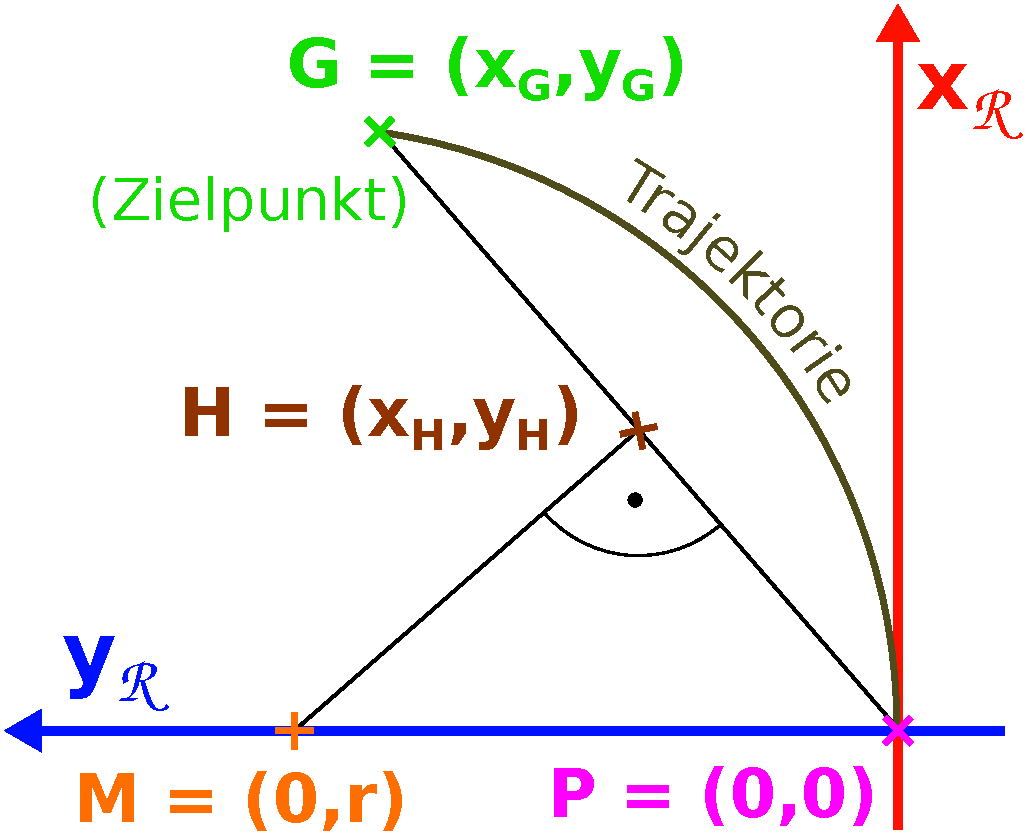
\includegraphics[width=0.8\textwidth]{regelung_lenkwinkel_radius.pdf}
  \caption{Visualisierung zur Bestimmung des Kreisradius aus dem gegebenen Zielpunkt in Roboterkoordinaten}
  \label{fig:regelung_lenkwinkel_radius}
\end{figure}

Es lassen sich zwei Hilfsgeraden \( \mathrm{g_1} \) und \( \mathrm{g_2} \) aufstellen. \( \mathrm{g_1}\) verläuft durch die Position des Roboters \pnt{p_0} sowie den Zielpunkt \gls{lat:zp} und stellt somit die Sehne des Kreisbogens der geplanten Trajektorie dar. Die Mittelsenkrechte dieser Sehne bildet die Gerade \( \mathrm{g_2} \).

\begin{eqnarray}
\text{Gerade } \mathrm{g_1}: \quad \gls{y} & = & {\gls{lat:anstieg}}_{\gls{lat:zp}} \cdot \gls{x} 	\\
\text{Gerade } \mathrm{g_2}: \quad \gls{y} & = & {\gls{lat:anstieg}}_h \cdot \gls{x} + {\gls{lat:achsenabschnitt}}_h  \label{eq:regelung_lenkwinkel_geradengleichung2}
\end{eqnarray}

Für den Schnittpunkt \pnt{h} gilt

\begin{eqnarray}
h_x & = & 0.5 \cdot {\gls{lat:zp}}_{\gls{x}} 	\\
h_y & = & 0.5 \cdot {\gls{lat:zp}}_{\gls{y}}
\end{eqnarray}

und für die Steigungen der Geraden gelten

\begin{eqnarray}
 {\gls{lat:anstieg}}_{\gls{lat:zp}} = \frac{\Delta \gls{y}}{\Delta \gls{x}} & = & \frac{{\gls{lat:zp}}_{\gls{y}}}{{\gls{lat:zp}}_{\gls{x}}} 	\\
 {\gls{lat:anstieg}}_h = \frac{\Delta \gls{y}}{\Delta \gls{x}} & = & \frac{{\gls{lat:zp}}_{\gls{x}}}{-{\gls{lat:zp}}_{\gls{y}}}
\end{eqnarray}

Die \( {\gls{y}}^{\gls{lat:RoboterKOS}} \)-Achse und die Gerade \( \mathrm{g_2} \) stehen jeweils senkrecht auf dem Kreisbogen und müssen sich demzufolge im Kreismittelpunkt \( {\gls{lat:mp}}_{\gls{lat:zp}} \) schneiden. Da \( {\gls{lat:mp}}_{\gls{lat:zp}} \) auf der \( {\gls{y}}^{\gls{lat:RoboterKOS}} \)-Achse liegt ist die \( {\gls{x}}^{\gls{lat:RoboterKOS}} \)-Koordinate mit \glqq 0\grqq{} bereits bekannt. Damit steht der gesuchte Radius \gls{lat:rad} in der \( {\gls{y}}^{\gls{lat:RoboterKOS}} \)-Komponente des Mittelpunktes, was wiederum bedeutet, dass auch \( \gls{lat:rad} = {\gls{lat:achsenabschnitt}}_h \) gilt. Setzt man mit diesem Wissen den Punkt \pnt{h} in die Geradengleichung von \( \mathrm{g_2} \) \eqref{eq:regelung_lenkwinkel_geradengleichung2} ein, erhält man durch Umstellen die Formel~\eqref{eq:regelung_lenkwinkel_radius} für den Radius \gls{lat:rad}.

\begin{equation}
\gls{lat:rad} = {\gls{lat:achsenabschnitt}}_h = h_y - {\gls{lat:anstieg}}_h \cdot h_x = 0,5 \cdot \left( {q}_{\gls{y}} + \frac{{q_{\gls{x}}}^2}{q_{\gls{y}}} \right)
\label{eq:regelung_lenkwinkel_radius}
\end{equation}

Ausgehend von Gleichung~\eqref{eq:regelung_lenkwinkel_lenkwinkeltan} lässt sich nun der gesuchte Lenkwinkel mit Hilfe der Arcustangensfunktion bestimmen.

\begin{equation}
\gls{gre:lenkwinkel} = \arctan \left( \frac{\gls{lat:radstand}}{\gls{lat:rad}} \right)
%\label{eq:regelung_lenkwinkel_lenkwinkel}
\end{equation}